\documentclass[t]{beamer}
\usepackage{CJKutf8}
\usepackage{amsfonts}
    \usepackage{amsmath}
    \usepackage{amssymb}
    \usepackage{amsthm}
    \usepackage{enumerate}
    \usepackage{graphicx}
    \usepackage{layout}
    \usepackage{mathrsfs}
    \usepackage{fancyhdr}
    \usepackage{subfigure}
    \usepackage{tcolorbox}
    \usepackage{tikz-cd}
    \usepackage{color}
    \usepackage{pifont}
    \usepackage{verbatim}
    \usepackage{mathtools}
    \usepackage{float}
    \usepackage{bm}
    \usetheme{AnnArbor}
% \usetheme{Antibes}
\usecolortheme{beaver}

% 添加网址的命令
\usepackage{hyperref}
% 这是一个带链接文本的示例:\href{https://www.example.com}{点击这里访问网站}
% 普通的示例:\url{https://www.example.com}
% 表格
\usepackage{booktabs}
\usepackage{multirow}

% \setbeamertemplate{navigation symbols}{}

\usepackage{textpos}

\newcommand{\dif}{\mathrm{d}}
\newtheorem{thm}{{定理}}

% some common command
\newcommand{\mm}[1]{$ #1$\newline}
% \newcommand{\tuichu}{\Rightarrow}
% \newcommand{\li}[1]{\newline#1}



\newcommand{\analysis}[2]{\forall \mathcal{E}{#1},\exists \delta {#2},s.t.}
\newcommand{\denyanalysis}[2]{\exists \mathcal{E}{#1},\forall \delta {#2},s.t.}
\newcommand{\yield}{\Rightarrow }
\newcommand{\jj}{\newline}
\newcommand{\ff}[1]{$ #1$}   % math environment + newline
\newcommand{\fgn}[1]{\begin{equation}#1\end{equation}  }
\newcommand{\fg}[1]{$$ #1$$}   % math environment + newline 
\newcommand{\pf}{$proof.$\newline}
\newcommand{\ee}{\newline\ff{\Box}\newline}
\newcommand{\fenshi}[2]{\ff{\frac{#1}{#2}}}
\newcommand{\shenlue}{\vdots\jj}
\newcommand{\abs}[1]{{\left \lvert #1 \right\rvert}}
\newcommand{\loge}[1]{In ({#1})}
\newcommand{\logical}[2]{log_{#2}^{#1}}
\newcommand{\summary}[3]{$\sum_{{#1}={#2}}^{#3}  $}
\newcommand{\denjia}[2]{{#1}\Leftrightarrow {#2}}
\newcommand{\jihe}[3]{ {#1}  = \{ {#2} \mid {#3} \} }
\newcommand{\ve}[2]{\left\langle {#1},{#2}\right \rangle}
\newcommand{\dakuohao}[2]{\begin{array}{rcl}{#1}\end{array} \} \Rightarrow{#2}}
\newcommand{\sxb}[3]{#1^{#2}_{#3}}
\newcommand{\sss}[2]{#1^{#2}}
\newcommand{\xxx}[2]{#1_{#2}}
\newcommand{\bri}[1]{\uppercase\expandafter{\romannumeral#1}}
\newcommand{\ri}[1]{\romannumeral#1} 
\newcommand{\polynomial}[8]{#1_{#2}#6^{#7}+#1_{#3}#6^{#8}+...+#1_{#4}#6+#1_{#5} }
\newcommand{\newd}[4]{f[{#1}_{#2},{#4},{#1}_{#3}]}
\newcommand{\lb}[2]{\begin{align*}\begin{split}{#1}\{ {#2}\end{split}\end{align*}}
\newcommand{\tab}[1]{\begin{array}{ll} {#1}\end{array}}


% 向量乘积
\newcommand{\avg}[1]{\left\langle #1 \right\rangle}
% 偏微分方程
\newcommand{\difFrac}[2]{\frac{\dif #1}{\dif #2}}
\newcommand{\pdfrac}[2]{\frac{\partial{#1}}{\partial{#2}}}
% 不同章节
\newcommand{\one}[1]{\section{#1}}
\newcommand{\two}[1]{\subsection{#1}}
\newcommand{\three}[1]{\subsubsection{#1}}
\newcommand{\aone}[1]{\section*{#1}}
\newcommand{\atwo}[1]{\subsection*{#1}}
\newcommand{\athree}[1]{\subsubsection*{#1}}
% 大括号,左右都有
\newcommand{\lbra}[1]{\left\{  {\begin{matrix} #1 \end{matrix}}\right. } 
% 样式 括号前缀 + 括号 
\newcommand{\lbras}[2]{{#1}\left\{ {  {\begin{matrix} #2 \end{matrix}}}\right. } 
\newcommand{\rbra}[1]{ \left.  {\begin{matrix} #1 \end{matrix}} \right\}  } 
% 模长
\newcommand{\distance}[1]{\parallel #1\parallel }
% 等价
\newcommand{\equ}{\Longleftrightarrow }
% 共轭
\newcommand{\cja}[1]{\overline{#1}}
% 两个矩阵,上面是 方框[] 下面是线条| 中间是 无
\newcommand{\mtx}[1]{\begin{matrix}#1\end{matrix} }
\newcommand{\bmtx}[1]{\begin{bmatrix}#1\end{bmatrix} }
\newcommand{\vmtx}[1]{\begin{vmatrix}#1\end{vmatrix} }
% \newcommand{\table}[1]{\begin{array}[lr]{ccc} #1 \end{array}}

%输入普通字符
\newcommand{\ww}[1]{\text{#1}}

% 所有内容 直接头文件搞定
\newcommand{\everything}[1]{\begin{document}\begin{CJK*}{UTF8}{gkai}#1\end{CJK*}\end{document}}


% 存放代码(失败了)
\newcommand{\cccode}[1]{\begin{lstlisting}#1\end{lstlisting}}

% 改变特定行序列
\newcommand{\ttt}{\subsection{}}

% 嵌套序号
\newcommand{\eee}[1]{\begin{enumerate}#1\end{enumerate}}


% 模板里面的一些宏
\newcommand{\pdfFrac}[2]{\frac{\partial #1}{\partial #2}}
\newcommand{\OFL}{\mathrm{OFL}}
\newcommand{\UFL}{\mathrm{UFL}}
\newcommand{\fl}{\mathrm{fl}}
\newcommand{\op}{\odot}
\newcommand{\Eabs}{E_{\mathrm{abs}}}
\newcommand{\Erel}{E_{\mathrm{rel}}}
% 变化颜色
\newcommand{\red}{\textcolor{red}}
\newcommand{\blue}{\textcolor{blue}}



% 流程图需要用到的宏包
\usepackage{palatino}
\usepackage{tikz}
\usetikzlibrary{shapes.geometric, arrows}
\tikzstyle{startstop} = [rectangle, rounded corners, minimum width = 2cm, minimum height=1cm,text centered, draw = black, fill = red!40]
\tikzstyle{io} = [trapezium, trapezium left angle=70, trapezium right angle=110, minimum width=2cm, minimum height=1cm, text centered, draw=black, fill = blue!40]
\tikzstyle{process} = [rectangle, minimum width=3cm, minimum height=1cm, text centered, draw=black, fill = yellow!50]
\tikzstyle{decision} = [diamond, aspect = 3, text centered, draw=black, fill = green!30]
% 箭头形式
\tikzstyle{arrow} = [->,>=stealth]
% 4个非常重要 的新命令
\newcommand{\start}[2]{    \node (start) [startstop]{#1};\node (in1) [io, below of = start]{#2};\lin{start}{in1}{}}
\newcommand{\stopp}[3]{\node (out1) [io, below of= #1]{#2};\node (stop) [startstop, below of=out1]{#3};\lin{out1}{stop}{} }
\newcommand{\pro}[6]{    \node (#3) [process, #2 of=#1,xshift=#4 cm]{#5};}
\newpage
\newcommand{\lin}[3]{\draw [arrow] (#1) --node [above] {#3} (#2);}


\begin{document}
\begin{CJK*}{UTF8}{gkai}
% 一般第一页显示PPT标题以及作者信息

% \BackgroundPic{./Screenshot from 2022-04-20 16-31-08.png}

% 增加学校 前面
\addtobeamertemplate{title page}{}{
	\begin{tikzpicture}[remember picture,overlay]
		% \node[yshift=85pt,xshift=50pt]{\includegraphics[height=2cm]{Screenshot from 2022-04-20 16-51-21.png}};
\end{tikzpicture}
}


	\title{创建时间序列的指令微调的数据集合并进行微调}
	\subtitle {} %不需要
	\author{
		陈钶杰\, \\
		专业:计算数学\,
	} % 显示作者
	% \institute {学院:数学科学学院} % 设置学院机构	
	\date{\today}  % 显示日期
\titlepage

% 设置目录
\begin{frame}{目录}
\frametitle{目录}	
\tableofcontents  % 显示目录
\end{frame} 



\section{论文解读-具有内存的大型语言模型(LLM)在计算机上是通用的}  

\begin{frame}
	\frametitle{}
    \begin{itemize}
		\item 
		\textcolor{red}{摘要}
		\begin{itemize}
		\item 具有内存的大型语言模型(LLM)在计算上是通用的.然而,主流LLM并没有充分利用记忆,其设计深受生物大脑的影响。由于其近似性和容易积累错误,传统的神经记忆机制无法支持LLM来模拟复杂的推理。在本文中,我们从现代计算机体系结构中寻求灵感,用符号记忆来增强LLM,用于复杂的多跳推理。这样的符号内存框架被实例化为LLM和一组SQL数据库,其中LLM生成操作SQL数据库的SQL指令。我们在需要复杂推理的合成数据集上验证了所提出的记忆框架的有效性。
		\end{itemize}
	\end{itemize}
\end{frame}

\begin{frame}
	\frametitle{introduction}
		\eee{
			\item 尽管LLM在理解和产生与情境相关的反应方面取得了重大进展,但它们也有局限性。其中一个主要挑战是,与语言模型的多回合交互会生成大量令牌,这很容易超过LLM的输入令牌限制。例如,GPT-4(32K)只能处理32000个令牌。随着交互的进行,LLM必须维护上下文信息(例如,用户输入和先前的响应),并根据累积的数据生成响应。然而,简单地将所有上下文信息串联起来并将其填充到LLM中,很容易超过LLM的处理能力并积累错误,导致模型失去对对话的跟踪,并产生不太准确的响应。
			\item 已经探索了一些神经记忆机制(Wu等人,2022a;Khattab等人,2022;Zhong等人,2022),以克服LLM的有限令牌输入问题。存储器组件充当来自先前交互的相关信息的存储和检索系统。然而,用传统的神经记忆增强LLM通常会导致在记忆中存储、检索和操作历史信息的困难,尤其是对于需要复杂多跳推理的任务。两个主要原因是(a)它们没有以结构化的形式存储历史信息;(b) 他们对存储在存储器中的信息的处理不是象征性的,因为他们都依赖于一些向量相似性计算,这可能是不准确的,从而导致错误的积累。
			\item 为了解决上述问题,我们建议使用数据库作为LLM的新型符号存储器。整个框架名为ChatDB。如图1所示,ChatDB由两个组件组成:LLM控制器及其内存。LLM控制器可以是任何常用的LLM(OpenAI,2023;Touvron等人,2023,Du等人,2022;Zeng等人,2022),并且负责控制对存储器的读取和写入操作。LLM的存储器可以是符号的或非符号的,或者两者的组合,负责存储历史信息并在需要时提供信息以帮助LLM响应用户输入。在ChatDB中,我们专注于使用数据库作为符号存储器,它允许通过执行符号语言(即SQL语句)来结构化存储历史信息。这些SQL语句是由LLM生成的。在需要精确记录、修改、查询、删除和分析历史数据的场景中,将数据库合并为符号存储器尤其有用。例如,商店经理需要维护日常销售记录,而使用纯文本或矩阵作为内存是不合适的(Chen et al.,2023)。然而,使用数据库作为外部符号存储器是非常合适的。该数据库使用SQL语句实现准确的操作,包括数据插入、删除、更新和选择。因此,使用数据库作为外部符号存储器可以确保管理和操作历史数据的准确性和效率,从而显著提高LLM在需要高精度和长期数据记录和处理的场景中的性能。
			\item 在ChatDB框架中,我们提出了记忆链(CoM)方法来更有效地操纵外部符号记忆,从而进一步增强LLM的推理能力。记忆链方法将用户输入转换为一系列中间的记忆操作步骤,这些步骤会产生最终结果。通过记忆链方法,将复杂的问题分解为多个步骤的记忆操作,大大降低了解决问题的复杂性。在ChatDB中,每个中间步骤都涉及一个或多个SQL语句。
			\item 我们的ChatDB为LLM领域做出了一些贡献。首先,我们建议用数据库作为其外部符号存储器来扩充LLM,允许历史数据的结构化存储,并使用SQL语句实现符号和复杂的数据操作。其次,我们的内存链方法通过将用户输入转换为多步中间内存操作来实现有效的内存操作,这增强了ChatDB的性能,使其能够处理复杂的多表数据库交互,并提高了准确性和稳定性。
			最后,我们的实验表明,用符号内存增强LLM可以提高多跳推理能力,防止错误积累,从而使ChatDB在合成数据集上显著优于ChatGPT。
		}
\end{frame}

\begin{frame}
	\frametitle{相关工作}	
	\eee{
		\item 记忆增强的大型语言模型(LLM)。LLM,如GPT-4(OpenAI,2023)和PaLM 2(Anil等人,2023年),已经证明了强大的推理和决策能力。然而,LLM经常受到其有限的上下文窗口大小的阻碍(例如,GPT-4只能处理32K令牌)。记忆增强LLM(Wu等人,2022a,b;Zhong等人,2022;Lewis等人,2020;Guu等人,2020年;Park等人,2023;Khattab等人,2022年;Izacard等人,2022)包含了一个记忆模块,该模块防止模型忘记关键信息,并允许其处理超过上下文窗口大小的长文本输入。在上下文学习中增强检索(Khattab等人,2022)使用检索模型(RM)来检索可以作为提示插入LLM中的相关信息。例如,Auto GPT 3和Generative Agents(Park等人,2023)利用内存模块直接存储文本提示,允许代理跟踪其历史记录。然后将过去的提示和当前的提示输入到LLM中进行处理。
		神经图灵机(NMT)(Graves et al.,2014),它将递归神经网络(RNN)与外部可训练的记忆资源结合在一起,并学习与梯度下降的记忆模块交互。门控图序列神经网络(GGS-NN)(Johnson,2017)构造和修改图,并利用图产生合理的输出。递归记忆变换器(RMT)(Bulatov et al.,2022)在输入和输出序列中引入额外的记忆标记,以存储、处理和交换长序列片段之间的局部和全局信息,然后训练模型来控制记忆操作和序列表示处理。
		\item 与LLM进行推理。众所周知,LLM在复杂的推理任务中很吃力。以前的方法侧重于结合专门设计的监督信号或微调,以增强语言模型的推理能力(Pi˛ekos et al.,2021;Ran等人,2019;Andor等人,2019年;Cobbe等人,2021;Chen等人,2022)。最近的方法主要是通过上下文学习来提高语言模型的推理能力(Brown et al.,2020;Lester et al.,2021;Wei et al.,2022022;Wang et al.,2022)。其中最具代表性的是思想链(CoT)(Wei et al.,2022),它将解决样本问题的中间推理过程呈现给语言模型,大大增强了其推理能力。
		\item 具有数据库的LLM。LLM在生成代码方面表现出了令人印象深刻的能力,包括Python代码、Excel的执行命令和数据库的结构化查询语言(SQL)(OpenAI,2023)。ChatExcel4使用LLM生成Excel执行命令,简化了用户交互过程。BINDER(Cheng等人,2022)提出了一个框架,该框架将任务输入映射到与API绑定的编程语言(例如Python代码)中的可执行程序,以调用LLM来执行广泛的功能。SQL-PALM(Sun et al.,2023)提出了一种基于LLM的文本到SQL模型,使用基于执行的自洽提示方法,并在很大程度上优于以前的Text-2-SQL方法。虽然以前的工作在一定程度上涉及数据库,但我们提出的ChatDB系统与这些方法有很大不同。具体而言,ChatDB将数据库视为LLM的外部符号记忆模块,然后利用数据库读取和写入基本数据信息,通过记忆链增强推理过程,从而获得更准确的推理结果。
		\item 使用LLM的工具。从工具使用的角度来看,ChatDB也可以被视为一种利用数据库作为工具的LLM(Schick et al.,2023;Shen et al.,2021;Surís et al.,2020;Paranjape et al.,2022)。Toolformer(Schick et al.,2023)通过一系列的演示,指示语言模型可以调用一些API来利用外部工具来解决当前的问题。另一个代表作是Auto GPT 5,它使语言模型能够使用搜索引擎完成一系列令人印象深刻的任务。ChatDB使用数据库作为外部工具的优势在于,它允许语言模型维护更准确的记录并使用历史数据,从而解决更复杂的问题,尤其是那些需要准确历史数据进行推理的问题。
		}
\end{frame}


\begin{frame}
	\frametitle{ChatDB}
	在本节中,我们首先简要介绍任务的定义和设置。然后,我们描述了我们提出的ChatDB的总体框架。最后,我们深入研究了内存链方法的细节,它是ChatDB的主要组件。
	\eee{
		\item 任务定义:\\
		给定自然语言的用户输入和数据库中现有表的详细信息(如果没有现有表,则不需要),目标是操作符号存储器,即外部数据库,以满足用户的请求。
		例如,如果用户(例如,商店经理)命令是记录、修改、查询和删除特定数据,则相应的SQL操作应该是分别在适当的表中插入、更新、选择和删除相关数据。这些操作通常涉及数据库中的多个表	\item 框架概述:\\
		ChatDB框架由三个主要阶段组成:输入处理、内存链和响应摘要,如图2所示。算法1提供了ChatDB响应用户输入的整个算法过程的详细说明。
		\eee{
		\item 输入处理。如果响应用户输入需要使用内存,则ChatDB会生成一系列中间步骤,通过使用LLM来操作符号内存。否则,我们将直接使用LLM生成回复。
		\item 记忆链。ChatDB执行一系列中间内存操作步骤来与符号内存交互。
		ChatDB根据之前生成的一系列SQL语句,依次操作符号内存,包括插入、更新、选择、删除等操作。外部数据库执行相应的SQL语句,更新数据库,并返回结果。值得注意的是,在执行此操作之前,ChatDB会根据先前SQL语句的结果来决定是否更新内存操作步骤。ChatDB按照相同的过程执行下一步,直到完成对内存的所有操作。
		\item 响应摘要。ChatDB根据一系列记忆步骤的结果总结了对用户的最终响应。
		}
		\item 3.3记忆链思维链(Wei et al.,2022)强调将复杂推理分解为一系列中间步骤。
		记忆链(CoM)可以被视为通过提供符号记忆机制来支持与这些中间步骤相关联的存储来增强思想链的一种方式。
		记忆链的目的是提高LLM在处理符号记忆时的推理能力和鲁棒性。该方法包括将用户输入转换为一系列中间内存操作,使LLM能够以符号方式更准确有效地操作内存。操作符号内存的能力对于涉及与历史数据的复杂而准确的交互的真实世界应用程序尤其有价值,例如管理环境中的记录保存和数据分析。
		为了提高我们方法的性能和稳定性,我们采用了上下文学习(Brown et al.,2020),提供了记忆链步骤和思维链提示的几个序列的提示示例。强大而准确的内存链过程使LLM能够比符号内存更好地推理,并处理更复杂的场景。
		记忆链的优点有两个。首先,它使LLM能够更准确地执行复杂的数据库操作,增强了它们在符号内存上的多跳推理能力。其次,通过将复杂的操作分解为一系列中间内存操作,内存链方法增强了LLM在处理复杂的多表交互时的能力。这种方法使LLM能够更好地处理边缘情况和意外场景,使其成为现实应用中一种很有前途的方法。
		\item 与以前的记忆增强LLM的比较
		在本小节中,我们对ChatDB和最近使用内存模块增强基于Transformer的语言模型的方法进行了全面的比较。先前工作中提出的语言模型的记忆模块可以大致分为两种类型。第一种类型的记忆存储上下文,并使用检索模型从过去的互动中找到与当前对话最相关的内容,然后将其用作语言模型的提示(Khattab等人,2022)。我们将这种类型的内存称为基于提示的内存。第二种类型的方法利用额外的记忆标记或记忆矩阵作为记忆(Bulatov et al.,2022),我们称之为基于矩阵的记忆。我们基于以下方面将ChatDB与这些方法进行比较:
		\eee{
			\item 内存格式。这个方面涉及用于存储存储器的格式。ChatDB利用数据库作为内存。基于提示的存储器(Park等人,2023)存储相关的交互内容和/或其相应的向量嵌入。基于矩阵的记忆采用额外的可训练记忆标记(Bulatov等人,2022023)或可训练记忆矩阵(Graves等人,2014)。
			\item 支持的操作。此方面指的是操作内存所支持的操作。ChatDB支持在数据库内存中插入、删除、更新和选择数据等操作。基于提示的内存主要支持插入和选择操作,但不完全支持更新和删除。
			基于矩阵的内存支持读取(选择)和写入(插入、更新、删除)操作。然而,由神经网络执行的确切操作尚不明确。
			\item 内存存储。这个方面指的是数据存储在存储器中的格式,特别是它是否结构化。ChatDB使用数据库以结构化格式存储内存,而基于提示的内存和基于矩阵的内存都被视为半结构化的。原因是向量嵌入和记忆矩阵有特定的维度和大小,但每个单独的维度都没有特定的明确含义。
			\item 内存执行。这方面的重点是如何执行内存操作,特别是它们是否是符号操作。ChatDB使用SQL在其数据库内存上执行操作,SQL是一种符号语言,因此使其具有内在的符号性。基于提示的存储器使用向量嵌入基于相似性度量来执行选择,并且使用语言编码器来获得用于插入的向量嵌入。这两者都被视为非象征性处决。在基于矩阵的记忆增强LLM中,记忆操作完全由神经网络控制,从而导致非符号执行。
			\item 可解释性。这个方面指的是记忆的可解释性程度。在ChatDB中,内存以结构化和显式的格式存储,其操作是符号化的,从而实现了高水平的可解释性。在基于提示的存储器中,由于解释向量嵌入的固有挑战,可解释性通常是有限的。
			对于基于矩阵的记忆方法,由于记忆完全由神经网络隐式控制,因此可解释性程度较低。
			\item 状态跟踪。这个方面涉及存储器是否有效地跟踪LLM的当前状态。在ChatDB的情况下,其内存准确地跟踪LLM的当前状态。水果店实验作为一个演示,在处理完每个记录后,ChatDB的数据库内存会更新,以反映水果店的最新状态。这展示了ChatDB的内存如何有效地跟踪其当前状态。得益于符号内存执行,ChatDB的内存可以轻松回滚到任何所需的时间戳,从而提供更大的灵活性和可控性。在基于矩阵的内存方法中,内存由模型本身不断更新和更改,使其能够跟踪LLM的当前状态。然而,基于提示的记忆方法只是存储历史背景,只知道过去发生了什么,而不清楚当前的状态。
			通过研究这些方面,我们观察到与现有方法相比,ChatDB的独特特征和能力。ChatDB的优势突出了使用符号内存来增强LLM的优势。
		}
	}	
\end{frame}

\begin{frame}
	\frametitle{评估}
	% \textcolor{red}{仔细区分这些不同的人机接口}	
		评估在本节中,我们进行实验来评估使用数据库作为其符号记忆来增强LLM的有效性。我们的实验结果表明,ChatDB显著优于基线模型ChatGPT,突出了符号内存集成的优势。
		\eee{
			\item 实验设置如前所述:\\
			使用数据库作为符号存储器特别适合于需要精确记录和处理历史信息的场景,例如各种数据管理场景。为了适应ChatDB的用例并能够与其他模型进行定量比较,我们构建了一个模拟水果店管理的合成数据集。
			此外,为了评估模型的性能,我们收集了一组50个带有注释标准答案的问题。这些问题的难度各不相同,既有需要多跳推理的难题,也有只需要从历史数据中检索信息的难题。共有15个简单问题和35个难题。
			每个问题都由模型独立回答。
			\item 4.1.1模型配置聊天数据库。在ChatDB中使用的LLM是ChatGPT(GPT-3.5Turbo),并且超参数温度设置为0。我们使用MySQL数据库作为外部符号内存。
比较基准。我们使用ChatGPT(GPT-3.5Turbo)作为基准模型,最大令牌长度为4096。与ChatDB类似,我们将温度设置为0。
			\item 我们合成了一个水果店管理记录的数据集,称为“水果店数据集”。该数据集模拟了商店中的四种常见操作:购买、销售、更改价格和退货。我们确保所有历史记录都是有效的,不会遇到负库存等问题。我们生成了70个按时间顺序排列的记录,总计约3.3k个令牌,这在ChatGPT的最大令牌长度限制(4096个令牌)内。\\
			为什么我们要限制数据集的令牌长度?如果数据集的令牌长度超过了ChatGPT的最大令牌长度,则需要内存。然而,主流的基于向量嵌入的内存检索方法容易出错。这不可避免地导致ChatGPT的性能下降,这是不可取的。
因此,我们故意将数据集的令牌长度设计在ChatGPT的最大令牌长度内,以避免使用内存并最大限度地提高模型的性能。请注意,ChatDB的性能通常不受数据集的令牌长度的影响。因此,如果在数据集小时ChatDB优于ChatGPT,则表明在数据集大时ChatDB也优于内存增强的ChatGPT。
			\item 4.1.3处理记录对于ChatDB,第一步是初始化数据库。我们需要为特定的任务场景生成一个合理的数据库模式,并在数据库中创建表。数据库模式的生成可以手动完成,也可以使用LLM。接下来,对于数据集中的每个记录,ChatDB逐一处理它们。使用LLM控制器,ChatDB按照算法1操作外部数据库(即符号存储器)。我们提供了ChatDB对水果店数据集中四种常见操作的响应示例,即购买、销售、价格变化和退货,如图3所示。值得强调的是,ChatDB逐个处理记录,因此对记录总数不敏感。此外,ChatDB中数据库操作的每一步都是象征性的,没有错误。因此,理论上,ChatDB可以在不牺牲性能的情况下处理无限多的历史记录。然而,对于ChatGPT或现有的内存增强LLM,过长的历史记录会显著降低性能。在这个实验中,对于ChatGPT基线,由于记录不长,我们只是将其作为提示的一部分。
			\item 4.1.4回答问题在回答问题时,ChatDB不再要求记录成为提示的一部分。在处理记录之后,信息被存储在符号存储器中。按照算法1,ChatDB利用SQL语句执行一系列数据库查询(包括计算),以回答问题。另一方面,ChatGPT将记录作为提示的一部分,并直接询问问题。提示模板如图4所示。			
		}
\end{frame}

\begin{frame}
	result	
	\eee{
		\item 实验结果如表2所示,清楚地表明ChatDB以显著更高的精度优于ChatGPT。虽然ChatGPT能够回答简单的问题,但它在处理需要多跳推理和精确计算的难题方面做得不够。因此,ChatGPT对这些难题的准确率较低。相比之下,ChatDB显示出显著的高准确率,突出了利用数据库作为符号存储器的优势。这种方法不仅防止了错误积累,而且增强了LLM的多跳推理和精确计算能力。
		为了进行比较,我们在图5中给出了两个模型回答问题的几个例子。在所有这些例子中,ChatDB正确地回答了问题,而ChatGPT失败了。如图5(a)所示,ChatGPT在计算每笔销售交易的总价时经常出现错误。有时,公式是正确的,但计算是错误的,而其他时候,甚至公式是不正确的。此外,ChatGPT很难找到所有有效的销售事务,导致其应答过程中出现错误。这个问题在所有这些例子中都很常见,也很明显。此外,ChatGPT倾向于产生顺序错误,从而导致显著的错误积累。
		相比之下,ChatDB在这些例子中表现得相当不错。在记录的初始处理过程中,应用符号操作(即SQL操作)来操作数据库(即符号内存),确保所有信息以结构化形式存储在数据库中。在回答问题时,ChatDB会生成SQL语句来查询数据库。这三个例子分别展示了ChatDB在解决需要一个、两个和三个记忆链步骤的问题方面的有效性。我们可以观察到,ChatDB准确地回答了问题,记忆链的执行逻辑清晰,每一步都紧密相连,接近最终答案。
		从这些例子来看,ChatDB的优势体现在两个方面:1。通过记忆链方法,将复杂的问题分解为多个记忆操作步骤,简化了问题的复杂性。每个步骤的结果都被准确地存储为中间结果,并在后续步骤中使用,这大大有助于复杂的推理。
		2.符号记忆可以实现精确的运算和计算。ChatDB通过执行SQL语句将许多计算任务委托给外部数据库,确保了每一步的准确性,防止了错误的积累。
		总之,通过利用外部数据库作为符号内存,ChatDB在本实验中显著优于ChatGPT。
		
	}
\end{frame}

\begin{frame}
	conclusion
	\eee{
		\item 在本文中,我们介绍了ChatDB,这是一个用数据库形式的符号内存增强LLM的框架。
		我们展示了符号记忆和记忆链方法在增强复杂推理和防止错误积累方面的优势和能力。通过为中间结果提供精确的存储机制,符号存储器实现了准确可靠的操作。此外,使用诸如SQL之类的符号语言可以对存储的信息进行符号计算和操作。通过实验评估,我们观察到与ChatGPT相比,ChatDB的性能显著提高。ChatDB中符号存储器的集成大大增强了模型在管理设置中处理各种查询和推理任务的能力。这一改进突出了在LLM中利用符号记忆的好处和有效性。		
	}
\end{frame}


% \subsection{大模型微调需要多少数据}

% \begin{frame}
% 	\textcolor{red}{浅层对齐假说}	
%     \begin{itemize}
% 		\item 一个模型的知识和能力几乎完全是在预训练中学习的,而对齐则是教它在与用户交互时应该使用哪种子分布的格式。
% 	\end{itemize}
% 	% \textcolor{red}{微调数据规模并不需要那么多,就可以达到一个不错的效果}	
% 	% \begin{itemize}
% 	% 	\item 在1000个精心策划的例子上对一个强大的预训练语言模型进行微调,可以在广泛的提示中产生显著的,有竞争力的结果.
% 	% \end{itemize}
% 	\textcolor{red}{结论}	
% 	\begin{itemize}
% 		\item 多样性,高质量这两个数据上的问题一直被认定是决定模型性能的天花板。
% 		\item 在目前的绝大多数微调模型,都是靠着大力出奇迹来实现一个较好的性能,这也是过去几个月大家都在卷数据量的一个真实写照。
% 		\item 但是否想过,openai这种什么技能都能做到的模型,在多样性上应该做了大量的工作,并且在数据量上应该没有太大的追求。
% 		\item 所以,最近的风向变成,是否可以利用少量的数据就能取得差不多的效果,这样的话,努力的方向就可以变成多样性数据的挖掘上,这可能是openai走通但我们没想明白的地方。
% 	\end{itemize}
% \end{frame}

% \begin{frame}
% 	\frametitle{决定大模型能力的关键因素}
% 	\textcolor{red}{模型参数还是训练文本的大小?}
%     \begin{itemize}
% 		\item PalM2选择后者为主要路径,文本数量是训练其前身模型的5倍.
% 		\item 微软的新模型Bard和chat GPT类似的存在,也是非常的强大.
% 	\end{itemize}
% \end{frame}


\subsection{压缩即智能?}

\begin{frame}
	\frametitle{如果大语言模型具备越强的数据压缩能力,是否意味着它具备越强的AGI智能呢?}	
	\textcolor{red}{数据压缩:压缩即智能}
    \begin{itemize}
		\item GPT模型训练的过程就是在进行数据压缩,将输入的语句等以参数的形式保存.比如Large Language Model Meta AI(LLAMA)模型的数据压缩率在14倍左右.
		\eee{
			\item "最小描述长度原理"可以用来解释这个观点.
			\item 比如我输入一个长度为1万的质数序列"2,3,5,11,...",那么对于这个输入的最佳解释即要尽可能短而准确的描述这个序列,比如输出"从2开始的一万个连续质数".\\
			% 我的理解是"从2开始的一万个连续质数"即是LLM模型把输入转化成的参数.
		}
		\item LLM的这种数据压缩能力是无损的.\\
		\eee{
			\item 此模型能根据上文Context,给出的后续Next Token肯定会有错误,这些被预测错误的Token,其实就代表了LLM压缩数据的信息损失,这种损失是靠算术编码额外对信息进行编码来进行补偿,才达成数据的“无损压缩”效果.即有如下的公式:\\
			\item 数据无损压缩=LLM模型的有损数据压缩能力+算数编码的补偿能力
		}
	\end{itemize}
	% 	\textcolor{red}{最小描述长度原理}
	% 	\begin{itemize}
	% 		\item 假设有很多模型可以对手上的数据进行描述,那么最佳解释就是尽可能短且精确的描述.
	% \end{itemize}
	% \textcolor{red}{GPT模型学习知识的顺序?}
	% \begin{itemize}
	% 	\item 高频知识点
	% 	\item 通用知识点
	% 	\item 具体而非抽象的知识点
	% \end{itemize}
\end{frame}
\subsection*{模型差异}

\begin{frame}
	% \frametitle{大LLM模型和小LLM模型的差异}	
	\textcolor{red}{大LLM模型和小LLM模型的差异}	
	% {小LLM模型建立了一个粗粒度的,模糊的世界图像,而随着模型规模越来越大,大LLM模型建立起能表征更多细节信息的清晰度越来越高的世界图像.}	
    \begin{itemize}
		\item 小LLM模型建立了一个粗粒度的,模糊的世界图像,而随着模型规模越来越大,大LLM模型建立起能表征更多细节信息的清晰度越来
		越高的世界图像.
	\end{itemize}
	\textcolor{red}{回路竞争视角下的tuning}
	\begin{itemize}
		\item "回路竞争"猜想:如果从低向上激发过程中,我们希望的正确回路被激发,可以认为回路竞争胜利,则模型输出正确答案,而如果错误任务回路被激发,可以认为回路竞争失败,则模型输出错误答案。
		% \item 比如我给了一个机器翻译的任务,输入经过逐个层后输出,这个输入在最开始的几层,可能会和其他任务(比如文本分类)的回路重叠,通过不断前进,重叠会不断变少,越到上层这个重叠会越少,最终得到机器翻译的输出.
		\item 可能通过Fine-tuning操作,在模型内部建立起了Shortcut捷径,导致输入信息后,信息传输直接走了捷径,而绕过了很多本该要走的通路。
		% \eee{
			% \item Fine-tuning操作通过大量领域数据,强化了大语言模型解决这个任务的响应回路。这对于模型底层知识点影响估计不大,因为底层更多的是通用性比较强的特征,这个任务也需要,它修正的应该更多是上层的抽象知识节点,以及底层知识点到上层抽象知识点建立激发连接的通路。
			% \item 很可能通过Fine-tuning操作,在模型内部建立起了Shortcut捷径,导致输入信息后,信息传输直接走了捷径,而绕过了很多本该要走的通路。
			% \item 比如文本分类任务,这种任务内部逻辑应该很简单,估计就是建立起底层具体领域词汇知识点,到上层抽象类别概念知识点`的激发通路,所以很可能直接从最底层的知识点,到高层的类别概念知识点,建立起了一个很短的Shortcut捷径,其它的复杂回路都被这个捷径给 pass掉了,倒不一定是上层抽象知识点被改写了,很可能是通过走捷径被绕过去了。
		% }
		\item 对于instruct tuning就是创造了一条新的特殊的激活回路,输入命令自身形成的激活回路,建立起和对应任务回路的连接.
	\end{itemize}
\end{frame}


\subsection{高效微调数据的方法(PEFT)}

\begin{frame}
	\frametitle{大模型参数高效微调(PEFT)}	
	\textcolor{red}{PEFT主要的两类方法,不同的方法对 PLM 的不同部分进行下游任务的适配}
    \begin{itemize}
		\item Prompt-Tuning(Prefix-Tuning):在模型的输入或隐层添加k个额外可训练的前缀 tokens(这些前缀是连续的伪 tokens,不对应真实的 tokens),固定 PLM 的所有参数,只训练这些前缀参数;	
		\item Adapter-Tuning:则是在预训练模型内部的网络层之间添加新的网络层或模块来适配下游任务。比如在transformer中Multi-Head层和FFN层中间插入一个Adapter层,固定其他参数,只调整Adapter层的参数
	\end{itemize}
\end{frame}

% \begin{frame}
% 	\frametitle{Prefix-Tuning}	
% 	\textcolor{red}{具体步骤}	
%     \begin{itemize}
% 		\item Prefix-Tuning 在模型输入前添加一个连续的且任务特定的向量序列(continuous task-specific vectors),称之为前缀(prefix)。前缀被视为一系列“虚拟 tokens”,但是它由不对应于真实 tokens 的自由参数组成。与更新所有 PLM 参数的全量微调不同,Prefix-Tuning 固定 PLM 的所有参数,只更新优化特定任务的 prefix。因此,在生产部署时,只需要存储一个大型 PLM 的副本和一个学习到的特定任务的 prefix,每个下游任务只产生非常小的额外的计算和存储开销。	
% 		\item Fine-tuning 更新所有 PLM 参数,并且需要为每个任务存储完整的模型副本。Prefix-tuning 冻结了 PLM 参数并且只优化了 prefix。因此,只需要为每个任务存储特定 prefix,使 Prefix-tuning 模块化且节省存储空间。	
% 		\item 针对NLG任务的设计:\\
% 		NLG(Natural Language Generation)任务:NLG任务是指计算机生成自然语言文本的过程。它涉及将非语言输入(如数据、结构化信息或逻辑表示)转化为自然语言表达,以便人类可以理解。NLG任务的目标是生成具有语法正确性、连贯性和可读性的自然语言文本。常见的NLG任务包括文本摘要、机器翻译、对话生成、问题回答生成等。NLG在智能助理、自动生成报告、自动生成文章等领域具有广泛应用.

% 		NLG任务是将非语言输入转化为自然语言文本		
% 	\end{itemize}
% \end{frame}

% \begin{frame}
% 	\frametitle{P-Tuning}	
% 	\textcolor{red}{具体步骤}	
%     \begin{itemize}
% 		\item P-Tuning 的方法思路与 Prefix-Tuning 很相近,P-Tuning 利用少量连续的 embedding 参数作为 prompt 使 GPT 更好的应用于 NLU 任务,而 Prefix-Tuning 是针对 NLG 任务设计,同时,P-Tuning 只在 embedding 层增加参数,而 Prefix-Tuning 在每一层都添加可训练参数。
% 		\item NLU(Natural Language Understanding)任务:NLU任务旨在让计算机能够理解和解释自然语言输入。它涉及将人类语言转化为机器可以理解和处理的形式。NLU任务的目标是从输入文本中提取出意图、实体、关键信息或上下文,并对其进行语义解析和理解。常见的NLU任务包括命名实体识别、意图识别、情感分析、关系抽取等。NLU在对话系统、语音识别、自动问答和信息检索等领域具有重要作用。

% 		NLU任务是将自然语言转化为机器可以理解的形式		
% 	\end{itemize}
% \end{frame}

% \begin{frame}
% 	\frametitle{Prompt Tuning}	
% 	\textcolor{red}{具体步骤}	
%     \begin{itemize}
% 		\item Prompt Tuning 方式可以看做是 Prefix Tuning 的简化,固定整个预训练模型参数,只允许将每个下游任务的额外  个可更新的 tokens 前置到输入文本中,也没有使用额外的编码层或任务特定的输出层。如下图所示,在模型大小增加到一定规模时,仅仅使用 Prompt Tuning 就足以达到 Fine Tuning 的性能。
% 		\item T5 的 Model Tuning 实现了强大的性能,但需要为每个任务存储单独的模型副本。 随着模型规模的增加,对 T5 的 Prompt Tuning 与 Model Tuning 的性能相当,同时允许所有任务复用同一固定模型。Prompt Tuning 方法明显优于使用 GPT-3 的少样本 Prompt Design。
% 		NLU任务是将自然语言转化为机器可以理解的形式
% 	\end{itemize}
% \end{frame}


\subsection{自然语言在代码上所面临的一些问题}

\begin{frame}
	% \frametitle{自然语言在代码上的应用}	
	\textcolor{red}{代码生成大模型的挑战和机遇}	
    \begin{itemize}
		\item 理解能力:人类能够理解不同抽象层次的各种描述,相比之下,当前的 LLM 往往对给定的上下文敏感,这可能会导致性能下降.
		\item 判断能力:	人类能够判定一个编程问题是否被解决。当前模型不论输入什么都会给出答案,而且该答案正确与否都不能确定,这在实际应用中会存在一定的问题。
		\item 解释能力:人类开发人员能够解释他们编写的代码,这对教育的和软件维护至关重要。
		\item 自适应学习能力:当前的大型语言模型与人类之间的一个根本区别是它们适应新知识和更新知识的能力。
		\item 多任务处理能力:代码大模型可以应用到各种各样和代码相关的任务中,例如代码修复,代码搜索,代码审核等。甚至代码大模型可以解决所有可以形式化为代码形式的下游任务。
	\end{itemize}
	% \textcolor{red}{编辑代码的网站}	
	% \begin{itemize}
		% \item 为了持续跟踪代码生成大模型领域的实时进展,作者提供了一个任何人都可编辑的实时更新在线网站:\\
		% https://nl2code.github.io/
	% \end{itemize}	
\end{frame}

\subsection{经过微调的LLaMA在算术任务上的性能优于GPT-4}

\begin{frame}
	\frametitle{经过微调的LLaMA在算术任务上的性能优于GPT-4}
	\eee{
		\item 我们的模型在各种基本算术任务上实现了最先进的性能,包括加法、减法、乘法,以及正整数的除法.	我们展示了在综合生成的数据集上与GPT-4相比,在算术任务上微调的开源模型实现更高精度的潜力.
		\item 证明监督的可行性,单独的微调可以使LLM为某些基本算术任务生成直接答案,例如大量加法和减法,而不应用任何特殊技术。令人印象深刻的性能主要归功于LLaMA数字的一致标记化。
		\item 为了解决大量的乘法和除法问题,我们提出了一种新的分解方法方法基于任务的可学习性,利用基本的算术原理来确保人类的可解释性.
		\item 我们系统地调查了分解方法及其证明有效性。我们对分解步骤进行了彻底的实验在一个完全合成的环境中,通过减轻自然的许多难以控制的方面语言我们的实验设置提供了研究CoT和中间监督.
		\item 我们的端到端指令调优管道可以可以很容易地集成到现有的指令调优语言模型中,并可能增强他们对数学单词的数学推理问题。
	}
\end{frame}


\section{代码上的尝试}


\begin{frame}
	\frametitle{代码}
\begin{itemize}
	\item 使用t5-base(2.8亿参数量,大小为1.3G)数据进行指令微调
	\begin{itemize}
		\item 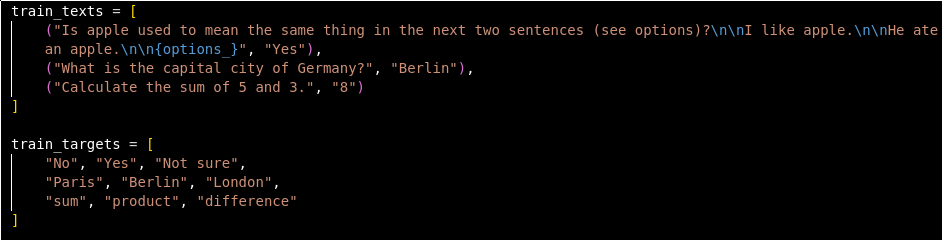
\includegraphics[scale=0.3]{png/p2.png}
		\item 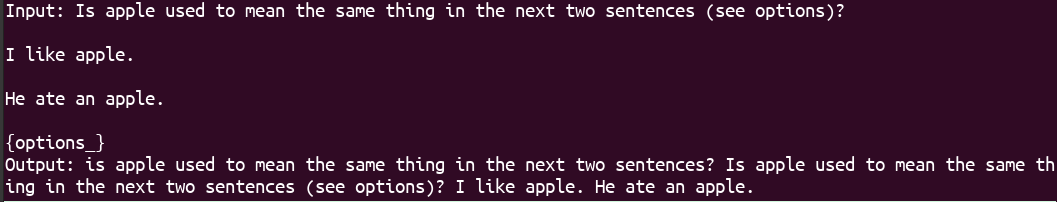
\includegraphics[scale=0.25]{png/p3.png}
		\item 只是重复了两遍.
	\end{itemize}

	
\end{itemize}
\end{frame}

\begin{frame}
	\frametitle{代码}
\begin{itemize}
	\item 时间序列的指令微调代码(t5\_finetuning.py)
	\eee{
		\item 程序有一些bug没跑通.
		\item 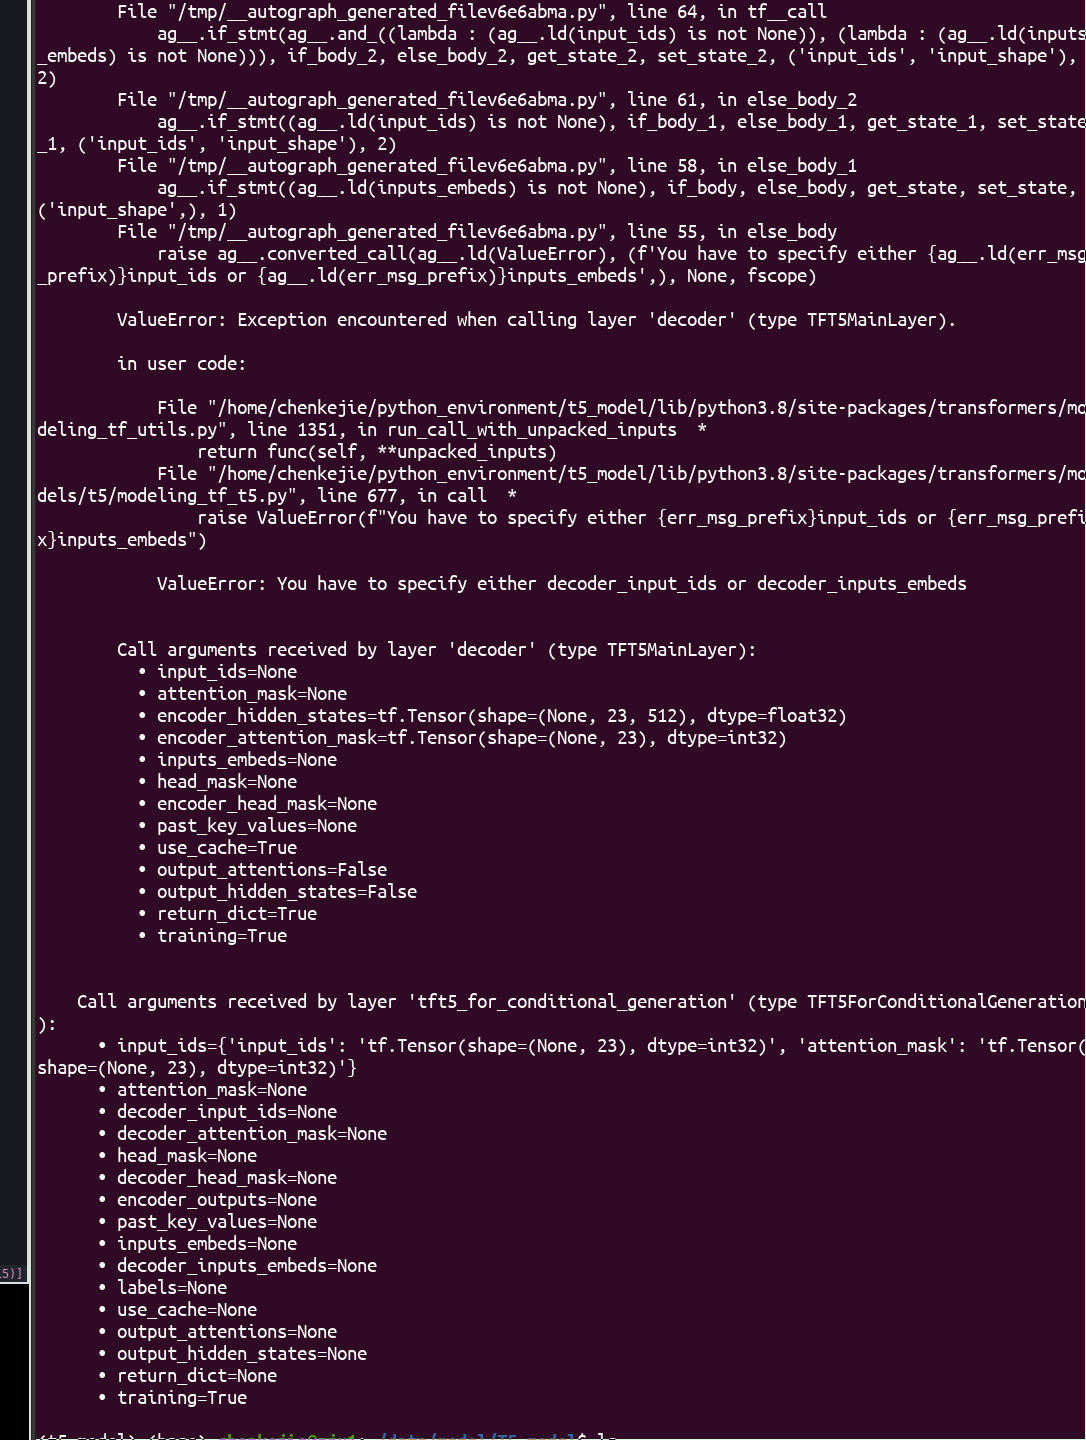
\includegraphics[scale=0.15]{png/p1.png}
				% \item TFT5ForConditionalGeneration模型是基于T5模型的条件生成模型,用于生成文本。在使用该模型时,需要提供decoder_input_ids或decoder_inputs_embeds参数来指定生成文本时的输入。
		% 根据报错信息,可以看到TFT5ForConditionalGeneration模型的调用参数中没有提供decoder_input_ids或decoder_inputs_embeds参数的值,导致报错。需要检查代码中关于生成文本输入的部分,确保提供了合适的参数。
		}
\end{itemize}
\end{frame}



\begin{frame}
	\frametitle{代码}
\begin{itemize}
	\item 时间序列的指令微调代码(t5\_finetuning.py)
	\eee{
		\item 在使用CUDA加速计算时,显存(GPU内存)不足以分配所需的张量。
		\item 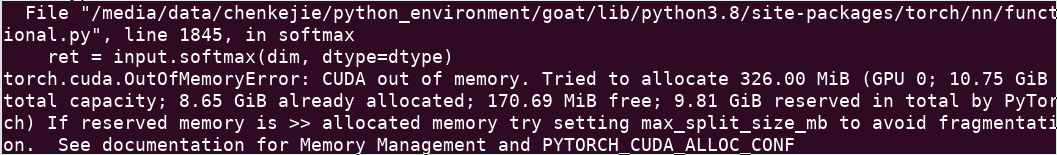
\includegraphics[scale=0.28]{png/bug.png}
		% \item TFT5ForConditionalGeneration模型是基于T5模型的条件生成模型,用于生成文本。在使用该模型时,需要提供decoder_input_ids或decoder_inputs_embeds参数来指定生成文本时的输入。
		% 根据报错信息,可以看到TFT5ForConditionalGeneration模型的调用参数中没有提供decoder_input_ids或decoder_inputs_embeds参数的值,导致报错。需要检查代码中关于生成文本输入的部分,确保提供了合适的参数。
		}
\end{itemize}
\end{frame}

\begin{frame}
	\frametitle{尝试运行如下几个程序:}
	\eee{
		\item Awesome-instruction-tuning:一个精心策划的开源指令调整数据集、模型、论文、资料库的列表。\\
		网址:\url{https://github.com/zhilizju/Awesome-instruction-tuning}
		\item stanford\_alpaca:该项目旨在建立和分享一个遵循指令的LLaMA模型。\\
		网址:\url{https://github.com/tatsu-lab/stanford_alpaca}
		\item Chinese-Vicuna:该项目旨在建立和分享遵循指令的中文LLaMA模型调整方法\\
		网址:\url{https://github.com/Facico/Chinese-Vicuna}
		\item FLAN:这个资源库包含了生成指令调谐数据集的代码。\\
		网址:\url{https://github.com/google-research/FLAN}
	}
\end{frame}


% 记得注释掉
% \begin{frame}
% 	\frametitle{llama模型}
% 	\eee{
% 		\item LLaMA (Touvron et al., 2023) 是一个集合
% 		训练有素的开源预训练语言模型使用公开数据集的数万亿个代币,并在许多方面实现了最先进的性能基准。
% 		先前的研究表明标记化对于 LLM 的算术能力很重要。 今天许多常用的子词标记化技术是不适合表示数字。 然而,美洲驼将每个数字拆分成一个单独的标记,从而确保数字的一致标记化,如附录 B 所示。
		
% 		语言模型的选择很重要我们的工作。 我们相信非凡的算术这项工作中展示的能力主要归功于 LLaMA 对数字。 我们通过实验验证其他LLM,例如 Bloom、OPT、GPT-NeoX 和Pythia,在相同的算术数据集上进行微调,无法匹配 LLaMA 的算术能力.
% 	}
% \end{frame}

% \begin{frame}
% 	\frametitle{test}
% 	\eee{
% 		\item LLaMA (Touvron et al., 2023) 是一个集合
% 		训练有素的开源预训练语言模型使用公开数据集的数万亿个代币,并在许多方面实现了最先进的性能基准。
% 		先前的研究表明标记化对于 LLM 的算术能力很重要。 今天许多常用的子词标记化技术是不适合表示数字。 然而,美洲驼将每个数字拆分成一个单独的标记,从而确保数字的一致标记化,如附录 B 所示。
		
% 		语言模型的选择很重要我们的工作。 我们相信非凡的算术这项工作中展示的能力主要归功于 LLaMA 对数字。 我们通过实验验证其他LLM,例如 Bloom、OPT、GPT-NeoX 和Pythia,在相同的算术数据集上进行微调,无法匹配 LLaMA 的算术能力.
% 	}
% \end{frame}



% 结束语
\section{}
\begin{frame}
	\frametitle{}
	\begin{center}
		\Huge{谢谢老师和同学的聆听!}
	\end{center}
\end{frame}


\end{CJK*}
\end{document}